\documentclass[oneside,final,14pt]{extreport}

%Общий вид и оформление
\usepackage{setspace}
\usepackage{indentfirst}
\usepackage{geometry}
\geometry{
	a4paper,
	left=20mm,top=15mm,right=20mm,bottom=15mm,
	headheight=0pt,headsep=0mm,foot=0pt,footskip=13mm,
	includeheadfoot
}
\linespread{1.05}
\raggedbottom
\sloppy
%Русский язык
\usepackage[nottoc,notlot,notlof]{tocbibind}
\usepackage{cmap}
\usepackage[utf8]{inputenc}
\usepackage[english, russian]{babel}


%Шрифты
\newcommand\veryhuge{\fontsize{55}{66}\selectfont}
\newcommand\verylarge{\fontsize{25}{30}\selectfont}
\newcommand\quitelarge{\fontsize{22.5}{27}\selectfont}
\newcommand{\garamond}{\fontencoding{T2A}\fontfamily{CormorantGaramond-LF}\selectfont}
\newcommand{\gillius}{\fontencoding{T1}\fontfamily{GilliusADFNoTwo-LF}\selectfont}

%Математические формулы
\usepackage{amsmath}
\usepackage{amsthm}
\usepackage{amssymb}
\usepackage{centernot}
\allowdisplaybreaks

\newcommand{\notimplies}{\centernot\implies}
\newcommand{\notimpliedby}{\centernot\impliedby}

%Таблицы
\usepackage{adjustbox}
\usepackage{hhline}
\usepackage{multirow}
\usepackage{caption}


%Графика
\usepackage[dvipsnames,svgnames]{xcolor}
\usepackage{graphicx}
\usepackage{tikz}
\usepackage{tikz-cd}
\usepackage{pgfplots}
\pgfplotsset{compat=1.16}
\usepgfplotslibrary{fillbetween}

%Заголовки глав и секций
\usepackage{titlesec}   
\titleformat{\section}
{\large\bfseries}{\thesection}{1em}{}   
\titleformat{\chapter}
{\Huge\bfseries}{}{0pt}{}
\titlespacing*{\chapter}
{0cm}{-\topskip}{1em}[0pt]

\usepackage{hyperref}
\hypersetup{
	colorlinks,
	citecolor=black,
	filecolor=black,
	linkcolor=blue,
	urlcolor=blue
}



%Прочие пакеты
\usepackage{relsize}
\usepackage{enumitem}
\usepackage[perpage]{footmisc}

%Обозначения математических операторов
\newcommand{\R}{\mathbb{R}}
\newcommand{\CC}{\mathbb{C}}
\newcommand{\I}{\mathbb{Z}}
\newcommand{\N}{\mathbb{N}}
\newcommand{\Rat}{\mathbb{Q}}


\begin{document}
	\tableofcontents
	
	\section{Постановка задачи}
	
	 Требуется решить разреженную систему матриц хранящихся в формате CSR.
	 
	  Для этого использовалась библиотека INMOST (C++). Ее функционал позволяет загрузить матрицу в указанном фрмате, создать переобуславливатель и запустить решатель по умолчанию (BiCGStab).
Требуется замерить время построения переобуславливателя, решения системы, и сделать это для значений параметра $drop\_tolerance = 0.1,~0.01,~0.001$.

	\section{Результаты}
	
	Способ замера времени: библиотека <chrono>. Код выполнялся на кластере ИВМ.

\begin{table}[h!]
	\centering
	\begin{tabular}{|c|c|c|}
		\hline
		$Drop\_tolerance$  & ILU Time [ms] & BiCGStab Time [ms]\\ \hline
		0.1 & 154 &  230 \\ 
		\hline
		0.01 & 429 & 104 \\
		\hline
		0.001 & 764 & 71\\
		\hline
	\end{tabular}
	\caption{$A\_g2\_1$}
	\label{table:1}
%\end{table}
\medskip
%\begin{table}[h!]
	\centering
	\begin{tabular}{|c|c|c|}
		\hline
		$Drop\_tolerance$  & ILU Time [ms] & BiCGStab Time [ms]\\ \hline
		0.1 & 3348 & 10166 \\ 
		\hline
		0.01 & 13354 & 4335 \\
		\hline
		0.001 & 35668 & 3551\\
		\hline
	\end{tabular}
	\caption{$A\_g2\_2$}
	\label{table:1}
%\end{table}
\medskip
%\begin{table}[h!]
	\centering
	\begin{tabular}{|c|c|c|}
		\hline
		$Drop\_tolerance$  & ILU Time [ms] & BiCGStab Time [ms]\\ \hline
		0.1 & 15844 & 79871 \\ 
		\hline
		0.01 & 13354 & 4335 \\
		\hline
		0.001 & 68362 & 27635\\
		\hline
	\end{tabular}
	\caption{$A\_g2\_3$}
	\label{table:1}
\end{table}

	
	\section{Портрет матрицы}
	\begin{center}
\begin{figure}[h]
	\centering
	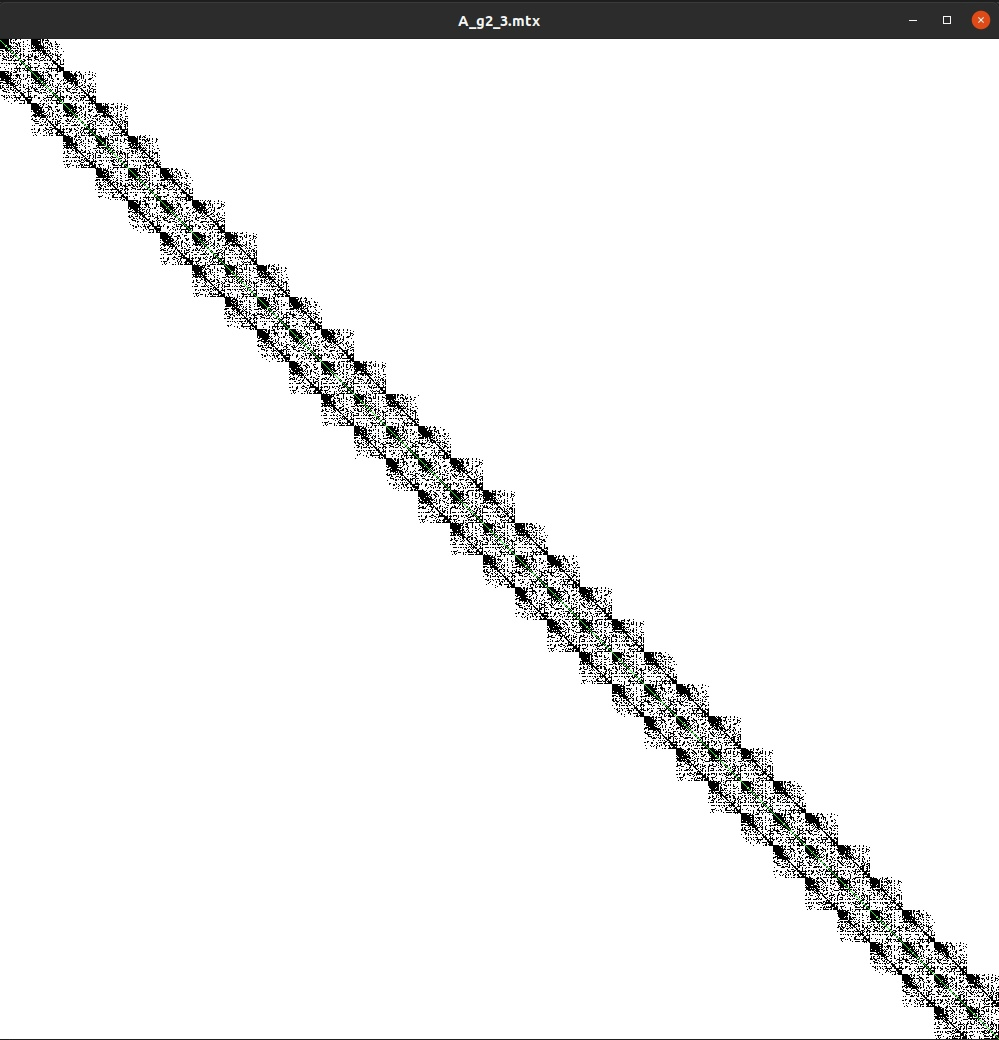
\includegraphics[scale=0.4]{YXQeLtRSUvc.jpg}
	\caption{Портрет матрицы}
	\label{fig:base-model-shema}
\end{figure}
\end{center}


\end{document}


%\begin{table}
%\begin{center}
%\begin{tabular}{|c|c|c|c|}
%\hline
%Size  & ILU Time [s] & PGMES Time [s] & Iterations\\ \hline
%4127 & 0.007 &  0.052  & 315 \\ \hline
%16527 & 0.025 & 7.450 & 584 \\
%\hline
%66159 & 0.090 & 99.836 & 1722\\
%\hline
%264751 & 0.351 & 733.469 & 3171\\
%\hline
%\end{tabular}
%\end{center}
%\end{table}
